\chapter{Implementacija i korisničko sučelje}
		
		\section{Korištene tehnologije i alati}
		
			 
			 Za izradu projekta koristili smo različite tehnologije, alate i platforme kako bismo učinkovito surađivali i razvili visokokvalitetnu aplikaciju. Za međusobnu komunikaciju unutar tima koristili smo aplikacije WhatsApp\footnote{\url{https://www.whatsapp.com/}} i Discord\footnote{\url{https://discord.com/}} što nam je omogućilo brz i jednostavan način dijeljenja informacija i dogovaranja.
			 
			 Sustav za upravljanje izvornim kodom bio je Git\footnote{\url{https://git-scm.com/}}, a repozitorij projekta smješten je na web platformi GitHub\footnote{\url{https://github.com/}}. Ovo nam je omogućilo sinkronizaciju rada, praćenje promjena i suradnju na kodu na učinkovit način. Za izradu UML dijagrama korišten je alat Astah UML\footnote{\url{https://astah.net/products/astah-uml/}}, pružajući jasnu vizualizaciju strukture i odnosa unutar projekta.
			 
			 Integrirano razvojno okruženje (IDE) koje smo koristili bilo je IntelliJ\footnote{\url{https://www.jetbrains.com/idea/}}, razvijeno u tvrtki JetBrains. IntelliJ je posebno prilagođen za rad s računalnim softverom napisanim u Javi, Kotlinu i Groovyju te pruža potporu za druge popularne jezike kao što su Python, JavaScript i TypeScript. To osigurava dosljedno iskustvo rada na različitim operativnim sustavima - Windows, macOS i Linux.
			 
			 Za backend aplikacije koristili smo Spring Boot\footnote{\url{https://spring.io/projects/spring-boot/}}, radni okvir baziran na Javi koji nudi autokonfiguraciju za olakšavanje početka razvoja, ali istovremeno omogućuje programerima da prilagode konfiguraciju prema potrebama.
			 
			 Frontend je implementiran pomoću Reacta\footnote{\url{https://react.dev/}}, biblioteke u JavaScriptu\footnote{\url{https://www.javascript.com/}} za izgradnju korisničkih sučelja. React se temelji na komponentama što je omogućilo razvoj složenih aplikacija s jasnom strukturom.\\
			 
			 Baza podataka projekta bila je PostgreSQL\footnote{\url{https://www.postgresql.org/}}, otvoreni sustav za upravljanje relacijskom bazom podataka. Konačno, aplikacija se nalazi na Renderu\footnote{\url{https://render.com/}}, oblak platformi kao usluzi, koja podržava različite programske jezike i omogućuje laku implementaciju i upravljanje modernim aplikacijama.
			 
			 Za ispitivanje sustava korišten je radni okvir Selenium\footnote{\url{https://www.seleniumhq.org/}} koji pruža automatsko testiranje kako bi se osigurala funkcionalnost i stabilnost sustava, a za ispitivanje komponenti JUnit\footnote{\url{https://junit.org/junit5/}}.
			 
			 Kombinacija ovih tehnologija i alata omogućila je timu učinkovit rad i uspješan razvoj aplikacije.
			
			
			\eject 
		
	
		\section{Ispitivanje programskog rješenja}
		
			 
			 Ispitivanje programskog riješena proveli smo na dva načina:
			 \begin{itemize}
			 	\item \textit{Ispitivanje komponenti - ostvareno pomoću JUnit testova u programskom jeziku Java}
			 	\item \textit{Ispitivanje sustava - ostvareno pomoću Selenium alata za automatizirano testiranje web aplikacija}
			 \end{itemize}
			 	
			 
			 
	
			
			\subsection{Ispitivanje komponenti}
			Ispitivanje komponenti bazira se na ispitivanjima funkcija programa kao što su broj poziva određene funkcije, što točno vraćaju funkcije nakon što se izvedu, izaziva li se neka iznimka itd.
			
			\begin{packed_enum}
				\item\textbf{Prvo testiranje testira kreiranje korisnika}
				
				\begin{quote}
						Provjeravamo funkcionalnost funkcija za kreiranje korisnika te koliko puta se koja funkcija pozvala.
						\begin{figure}[H]
							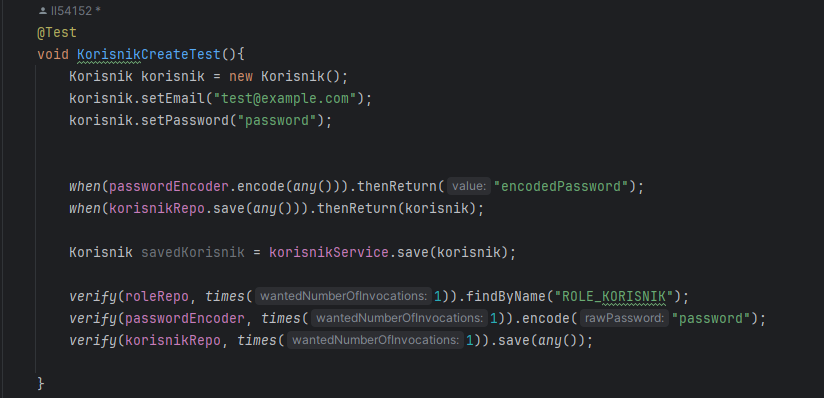
\includegraphics[width=\textwidth]{slike/JUnit1.png} %veličina u odnosu na širinu linije
							\caption{Prvo testiranje}
							\label{fig:JUnit1} %label mora biti drugaciji za svaku sliku
						\end{figure}
				\end{quote}
				
				
				\item\textbf{Drugo testiranje testira ulazak u konferenciju}
				
				\begin{quote}
					U drugom testiranju provjeravamo ulazak u konferenciju kao i sve funkcionalnosti vezanu uz nju.
					\begin{figure}[H]
						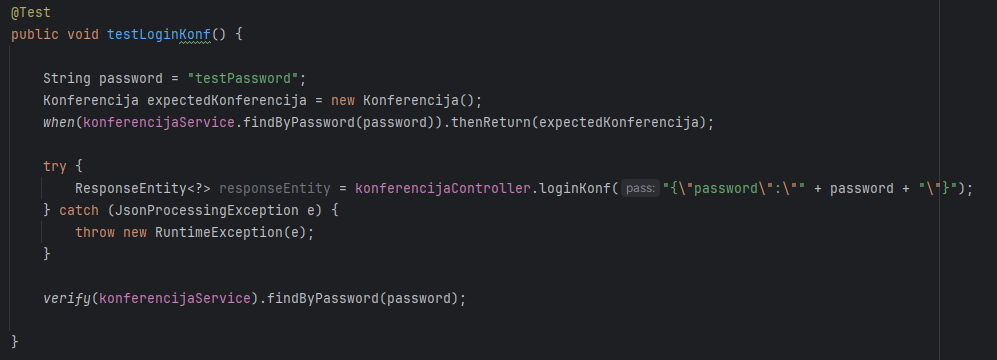
\includegraphics[width=\textwidth]{slike/JUnit2.png} %veličina u odnosu na širinu linije
						\caption{Drugo testiranje}
						\label{fig:JUnit2} %label mora biti drugaciji za svaku sliku
					\end{figure}
				\end{quote}
				
				\item\textbf{Treće testiranje testira neuspješan ulazak u konferenciju}
				\begin{quote}
					U trećem testiranju provjeravamo ponašanje naše aplikacije u slučaju neuspjelog ulaska u konferenciju kao i sve funkcionalnosti vezanu uz nju.
					\begin{figure}[H]
						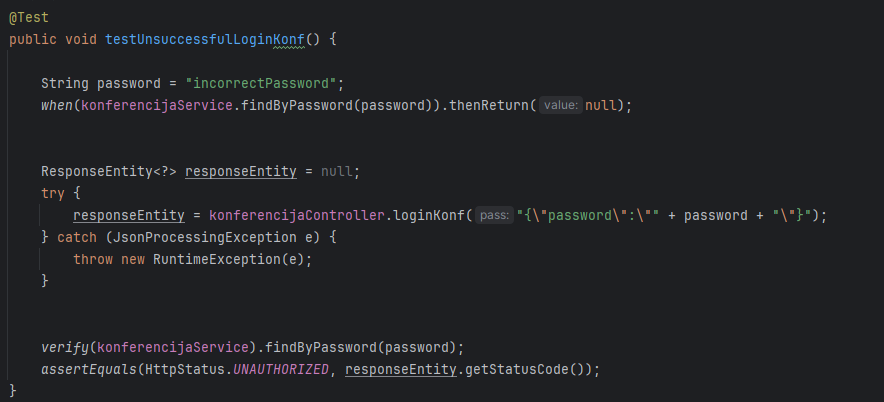
\includegraphics[width=\textwidth]{slike/JUnit3.png} %veličina u odnosu na širinu linije
						\caption{Treće testiranje}
						\label{fig:JUnit3} %label mora biti drugaciji za svaku sliku
					\end{figure}
				\end{quote}
				
				\item\textbf{Četvrto testiranje testira dohvat svih konferencija}
				\begin{quote}
					U četvrtom testiranju testiramo funkcionalnost dohvaćanja svih konferencija budući da je to jedna od ključnih funkcija prilikom kreiranja konferencije.
					\begin{figure}[H]
						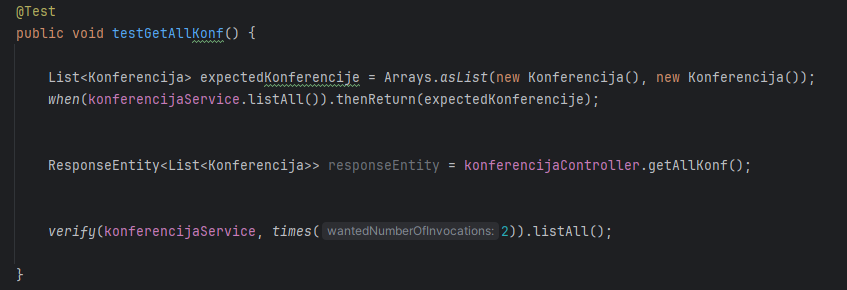
\includegraphics[width=\textwidth]{slike/JUnit4.png} %veličina u odnosu na širinu linije
						\caption{Četvrto testiranje}
						\label{fig:JUnit4} %label mora biti drugaciji za svaku sliku
					\end{figure}
				\end{quote}
				
				\item\textbf{Peto testiranje testira dohvat svih lokacije}
				\begin{quote}
					U petom testiranju testiramo funkcionalnost dohvaćanja lokacije koja je ključna za prikaz karte i vremenske prognoze.
					\begin{figure}[H]
						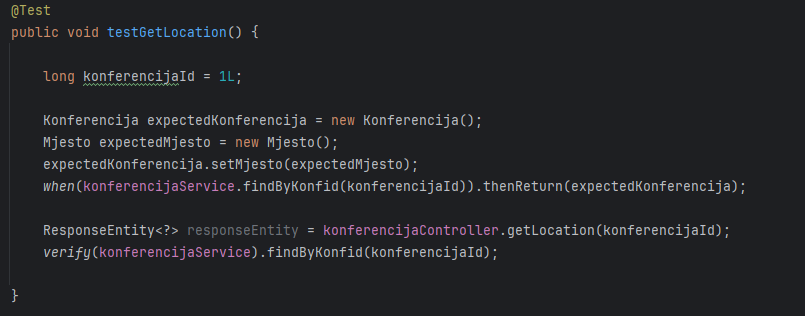
\includegraphics[width=\textwidth]{slike/JUnit5.png} %veličina u odnosu na širinu linije
						\caption{Peto testiranje}
						\label{fig:JUnit5} %label mora biti drugaciji za svaku sliku
					\end{figure}
				\end{quote}
				
				\item\textbf{Šesto testiranje testira kreiranje mjesta uz konferenciju}
				\begin{quote}
					U šestom testiranju testiramo funkcionalnost kreiranja i dodavanja mjesta nekoj konferenciji.
					\begin{figure}[H]
						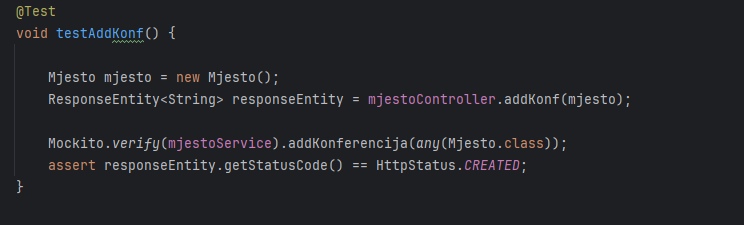
\includegraphics[width=\textwidth]{slike/JUnit6.png} %veličina u odnosu na širinu linije
						\caption{Šesto testiranje}
						\label{fig:JUnit6} %label mora biti drugaciji za svaku sliku
					\end{figure}
				\end{quote}
				
			\begin{figure}[H]
				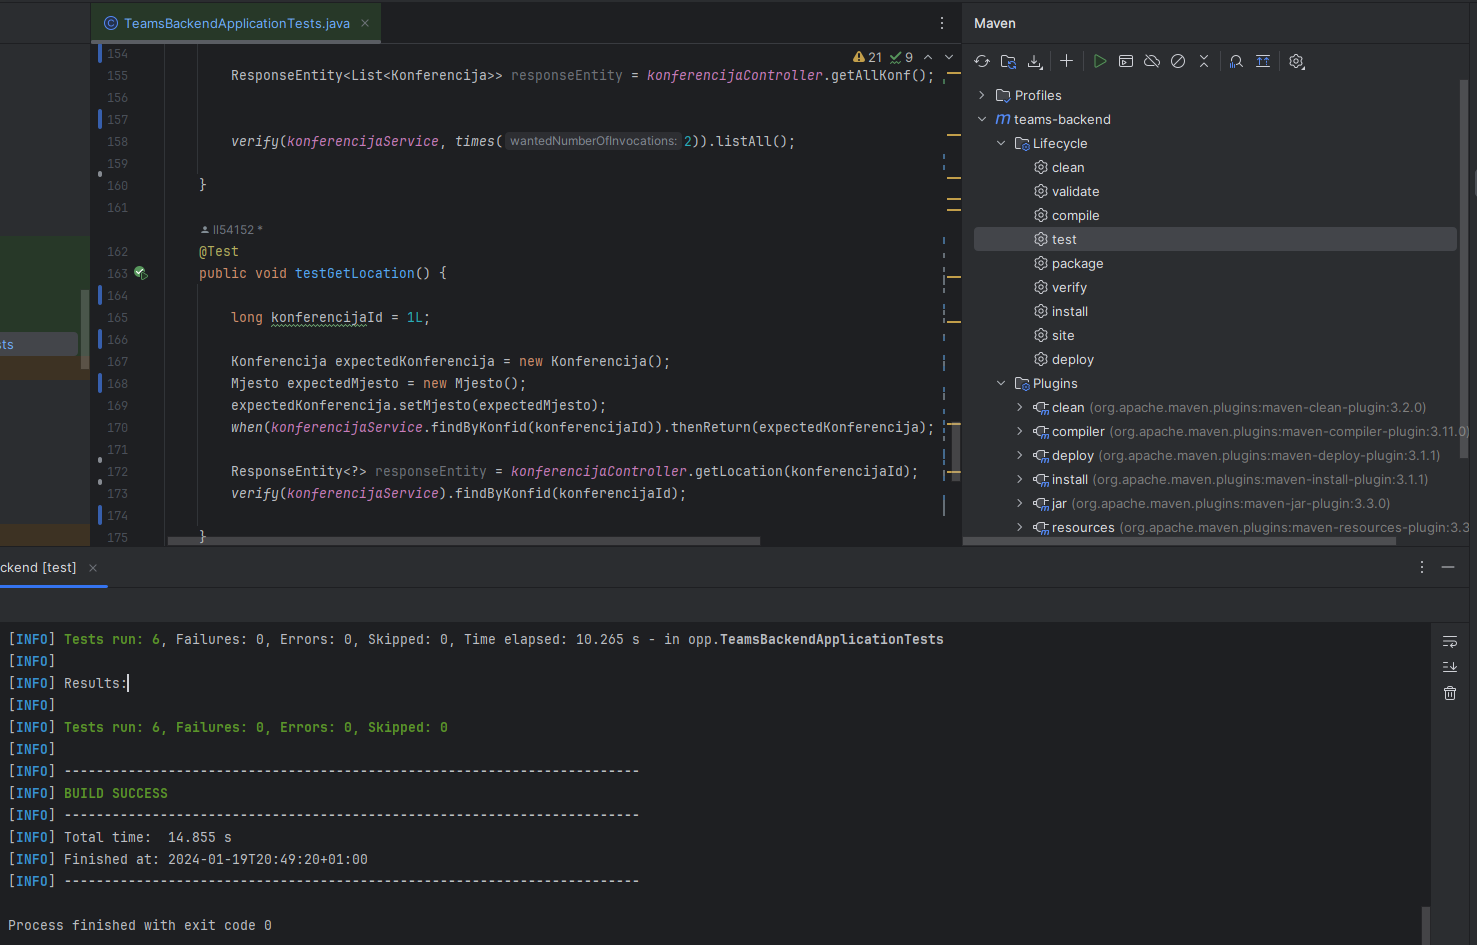
\includegraphics[width=\textwidth]{slike/JUnitAll.png} %veličina u odnosu na širinu linije
				\caption{Rezultati testova}
				\label{fig:JUnitAll} %label mora biti drugaciji za svaku sliku
			\end{figure}
			
				
			\end{packed_enum}
			
			
			
			\subsection{Ispitivanje sustava}
			Ispitivanje sustava proveli smo koristeći Selenium WebDriver i zadnju verziju FireFox web-preglednika. Selenium smo konfigurirali pomoću programskog jezika Java te je onda Selenium automatizirano testirao našu aplikaciju bazirajući se na naše testove. Za Selenium testiranje isključili smo reCAPTCHA.
	
			
			\begin{packed_enum}
				\item\textbf{Prvo testiranje testira registraciju korisnika}
				
				\begin{quote}
					Provjeravamo funkcionalnost registracije korisnika. U polja upisujemo podatke te se pritišće gumb nakon upisa. Ukoliko je test prošao, korisnik je uspješno stvoren i prijavljen u aplikaciju.
					\begin{figure}[H]
						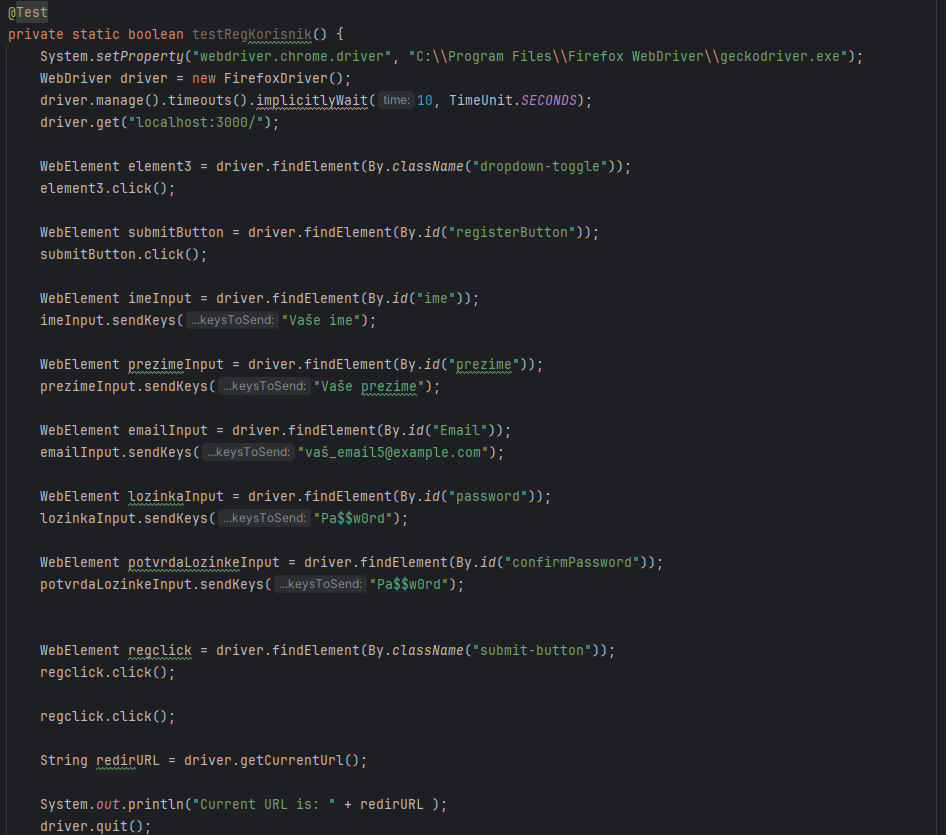
\includegraphics[width=\textwidth]{slike/Selenium1.png} %veličina u odnosu na širinu linije
						\caption{Prvo testiranje}
						\label{fig:Selenium1} %label mora biti drugaciji za svaku sliku
					\end{figure}
				\end{quote}
				
				
				\item\textbf{Drugo testiranje testira dodavanje konferencije}
				
				\begin{quote}
					U drugom testiranju provjeravamo dodavanje konferencije. Prije samog dodavanja konferencije administrator se mora prijaviti u sustav te nakon prijave administrator upisuje podatke za konferenciju te pritišće gumb za dodavanje. Ukoliko je test prošao, konferencija će biti dodana te će se prikazati poruka o uspješnosti našeg dodavanja.
					\begin{figure}[H]
						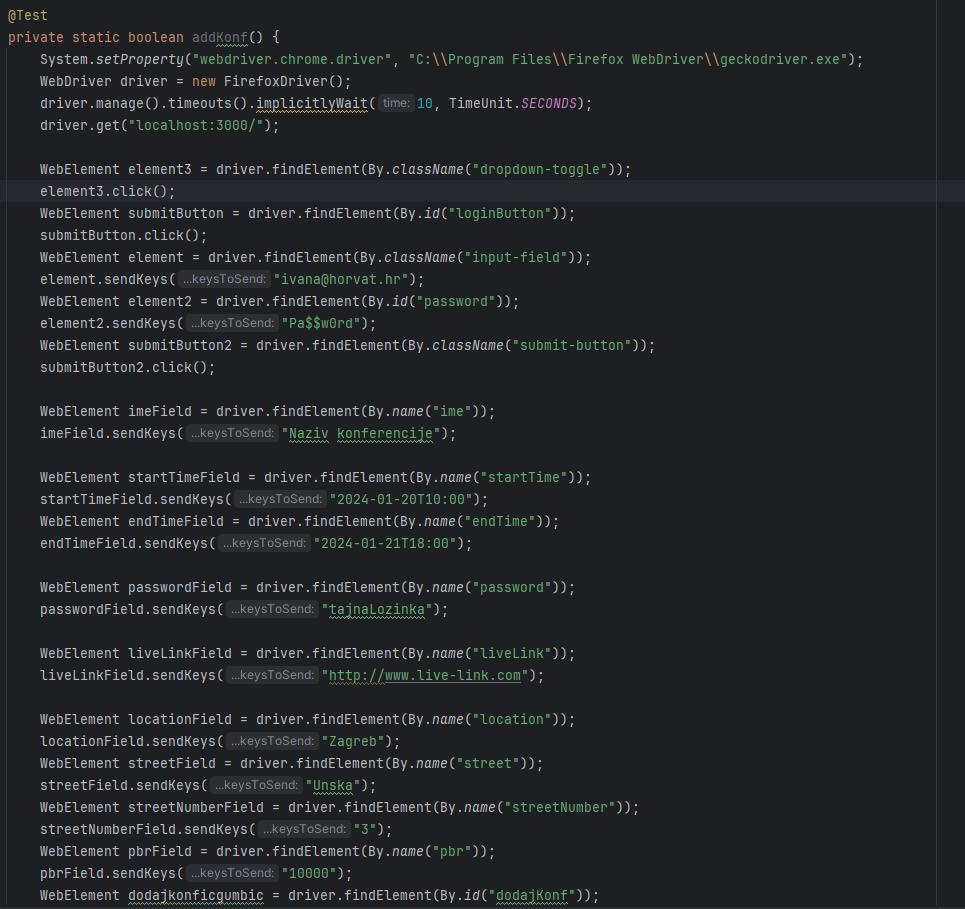
\includegraphics[width=\textwidth]{slike/Selenium2.png} %veličina u odnosu na širinu linije
						\caption{Drugo testiranje}
						\label{fig:Selenium2} %label mora biti drugaciji za svaku sliku
					\end{figure}
				\end{quote}
				
				\item\textbf{Treće testiranje testira prijavu korisnika}
				\begin{quote}
					U trećem testiranju provjeravamo prijavu korisnika. U prazna polja upisujemo potrebne podatke te na kraju pritišćemo gumb za prijavu. Ukoliko je test uspješan, vratit će nas na početnu stranicu.
					\begin{figure}[H]
						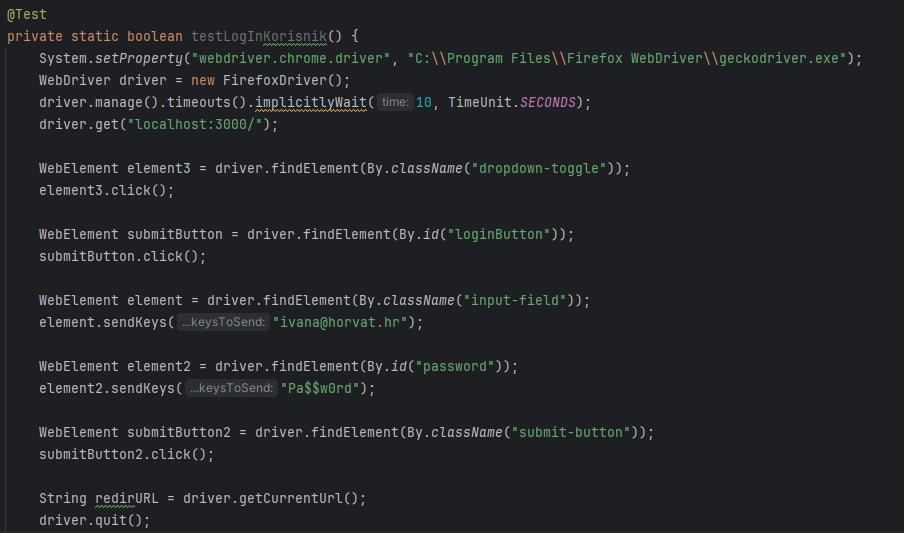
\includegraphics[width=\textwidth]{slike/Selenium3.png} %veličina u odnosu na širinu linije
						\caption{Treće testiranje}
						\label{fig:Selenium3} %label mora biti drugaciji za svaku sliku
					\end{figure}
				\end{quote}
				
				\item\textbf{Četvrto testiranje testira prijavu u konferenciju}
				\begin{quote}
					U četvrtom testiranju testiramo prijavu u konferenciju. Unutar polja za unos lozinke, upisujemo lozinku i pritišćemo gumb za prijavu. Ukoliko je test uspješan, aplikacija će nas vratiti na početnu stranicu konferencije.
					\begin{figure}[H]
						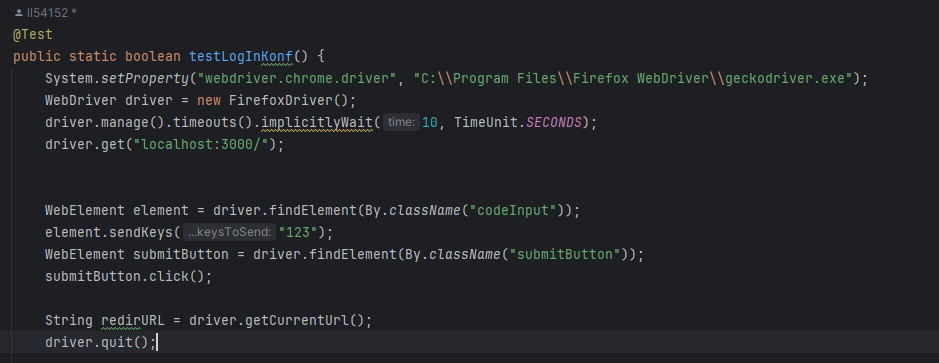
\includegraphics[width=\textwidth]{slike/Selenium4.png} %veličina u odnosu na širinu linije
						\caption{Četvrto testiranje}
						\label{fig:Selenium4} %label mora biti drugaciji za svaku sliku
					\end{figure}
				\end{quote}
				
			\end{packed_enum}
			
			\begin{figure}[H]
				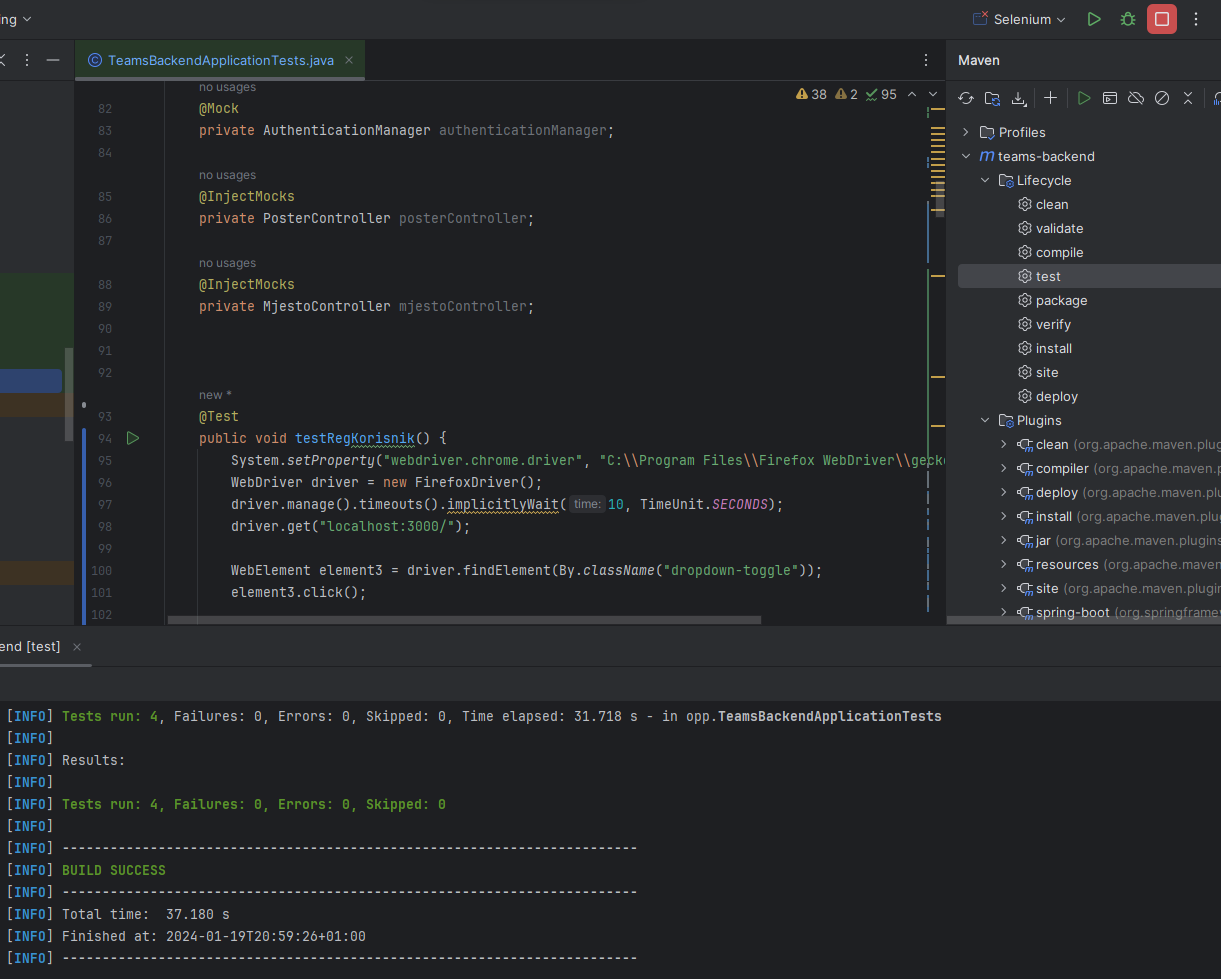
\includegraphics[width=\textwidth]{slike/SeleniumAll.png} %veličina u odnosu na širinu linije
				\caption{Rezultati testova}
				\label{fig:SeleniumAll} %label mora biti drugaciji za svaku sliku
			\end{figure}
			
			\eject 
		
		
		\section{Dijagram razmještaja}
			
			Dijagram razmještaja~\ref{fig:dijagramRazmjestaja} opisuje topologiju sklopovlja i programsku potporu koja se koristi u implementaciji sustava u njegovom radnom okruženju. Sustav je baziran na arhitekturi "klijent-poslužitelj". Poslužiteljsko računalo (Render) sadrži web poslužitelj na kojem se nalazi naša web aplikacija te sadrži poslužitelj baze podataka na kojemu je naša PostgreSQL baza podataka. Komunikacija između klijenta i poslužitelja obavlja se preko sigurnog kanala ostvarenog protokolom HTTPS.
			
			
			 \begin{figure}[H]
				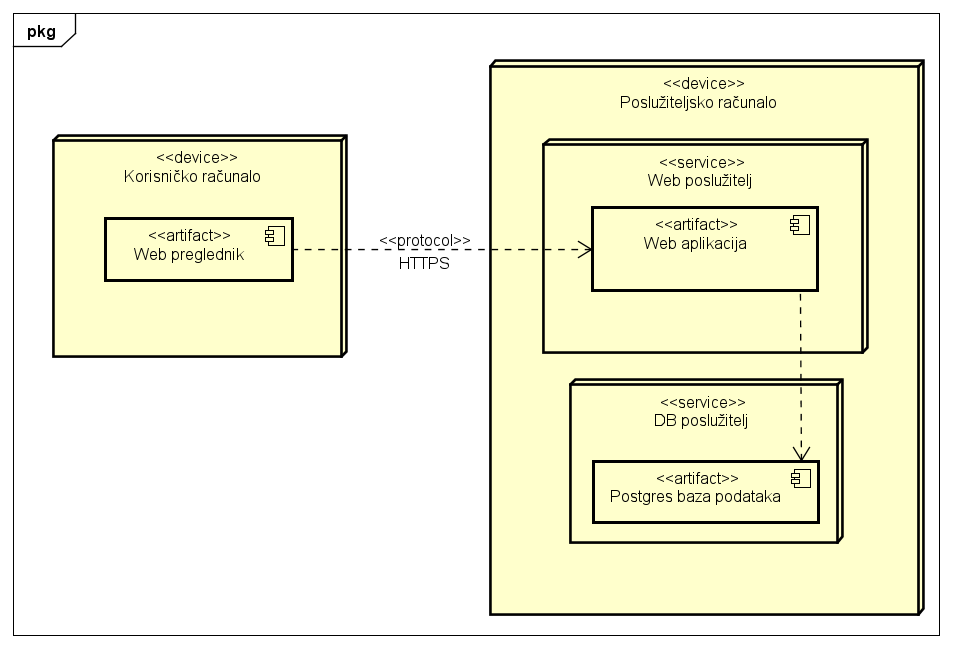
\includegraphics[width=\textwidth]{slike/dijagramRazmjestaja.PNG} %veličina u odnosu na širinu linije
				\caption{Dijagram razmještaja}
				\label{fig:dijagramRazmjestaja} %label mora biti drugaciji za svaku sliku
			\end{figure}
			
			
			\eject 
		
		\section{Upute za puštanje u pogon}
		
			Za puštanje aplikacije u pogon (eng. deployment) koristili smo web stranicu Render.
			Prema uputama danim na GitHub repozitoriju tvrtke CROZ \url{(https://github.com/progi-devops/)} pripremili smo naš sustav za puštanje u pogon.
			Kako bismo mogli koristiti usluge servisa Render, prvotno smo se morali prijaviti u sustav, a to smo učinili pomoću istih podataka s kojima smo stvorili GitHub repozitorij na kojemu držimo i održavamo naš projekt te njegov kod. Prvotno se podiže virtualna baza, a nakon nje potrebno je namjestiti skripte (navedene u package.json dokumentu i Dockerfile dokumentu) koje se izvode prilikom izgradnje rješenja projekta te prilikom samog pokretanja tog izgrađenog rješenja. To vrijedi i za pripremu "backend" i "frontend" dijela. Također, za "frontend" dio, u uputama se mogu pronaći koraci kako osigurati neometano lokalno pokretanje aplikacije bez obzira na novododane datoteke. Pri podizanju baze nije potrebno unositi gotovo nikakve podatke, već samo vrstu bazu kojom se koristimo (u našem slučaju PostgreSQL) te vremensku zonu kojoj pripadamo. Nakon toga Render nam povratno pruža sve potrebne informacije koje nam trebaju za lokalno spajanje na virtualnu bazu te povezivanje "backenda" na nju. Nakon toga moramo pustiti u pogon "backend" dio aplikacije kako bismo dobili URL na koji će naš "frontend", pušten u pogon, slati zahtjeve i s kojega će primati odgovore. Dockerfile koji nam je potreban za puštanje u pogon kreirali smo po uzoru na dani Dockerfile sa već spomenutog GitHub repozitorija uz manje preinake kod podataka vezanih za povezivanje na bazu. Isto vrijedi za package.json dokument te app.js. Također, bitno je istaknuti da Render prilikom puštanja u pogon koristi prethodno zadanu granu s odabranog repozitorija s koje potom uzima kod koji konkretno pušta u pogon. Tako prilikom svakog novog postavljanja promjena (eng. commit and push) na odabranu granu na Render se servisu automatski ponovno pušta u pogon kompletna aplikacija (osim baze podataka) s novim promjenama.
			
			\begin{figure}[H]
				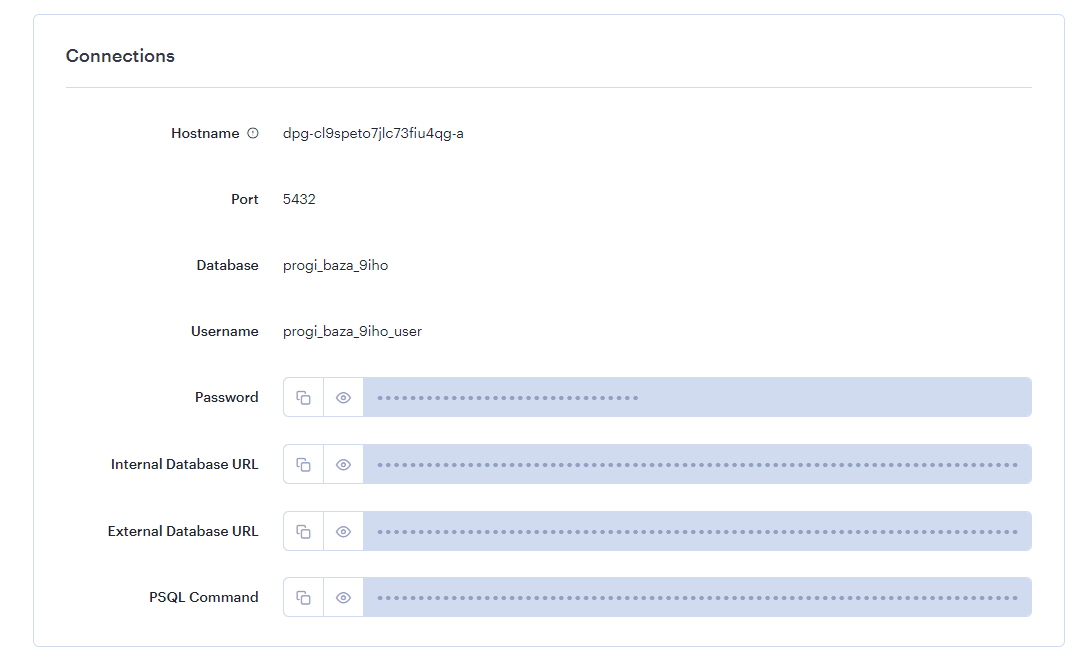
\includegraphics[width=\textwidth]{slike/DB_podatci.png} %veličina u odnosu na širinu linije
				\caption{Generirani podatci za povezivanje na bazu}
				\label{fig:DB_podatci} %label mora biti drugaciji za svaku sliku
			\end{figure}
			
			\begin{figure}[H]
				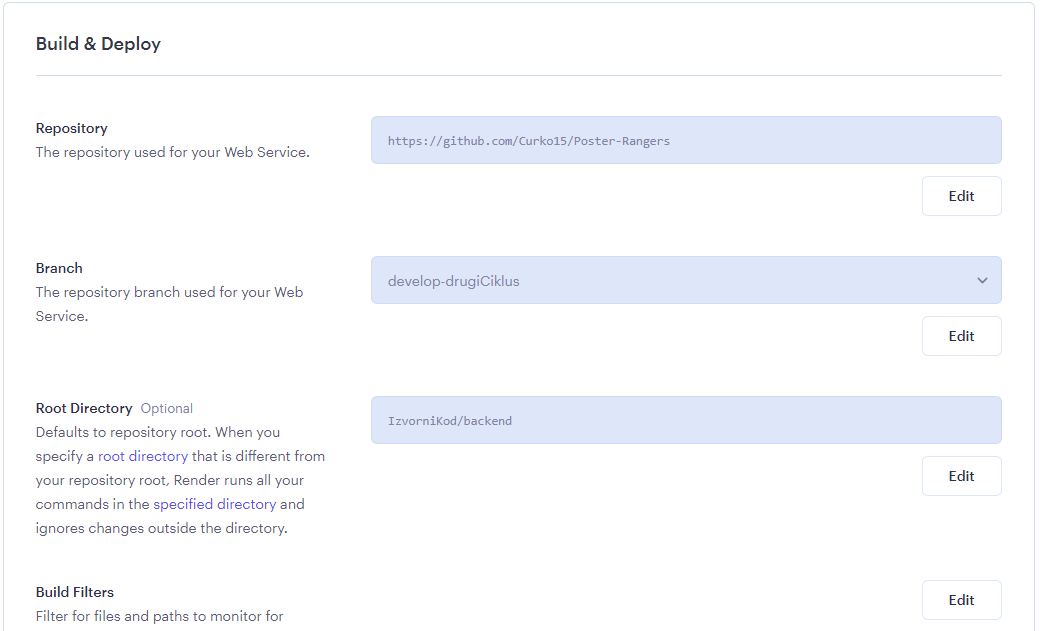
\includegraphics[width=\textwidth]{slike/BE_setup.png} %veličina u odnosu na širinu linije
				\caption{Postavljanje repozitorija, grane te direktorija za "backend"}
				\label{fig:BE_setup} %label mora biti drugaciji za svaku sliku
			\end{figure}
			
			\begin{figure}[H]
				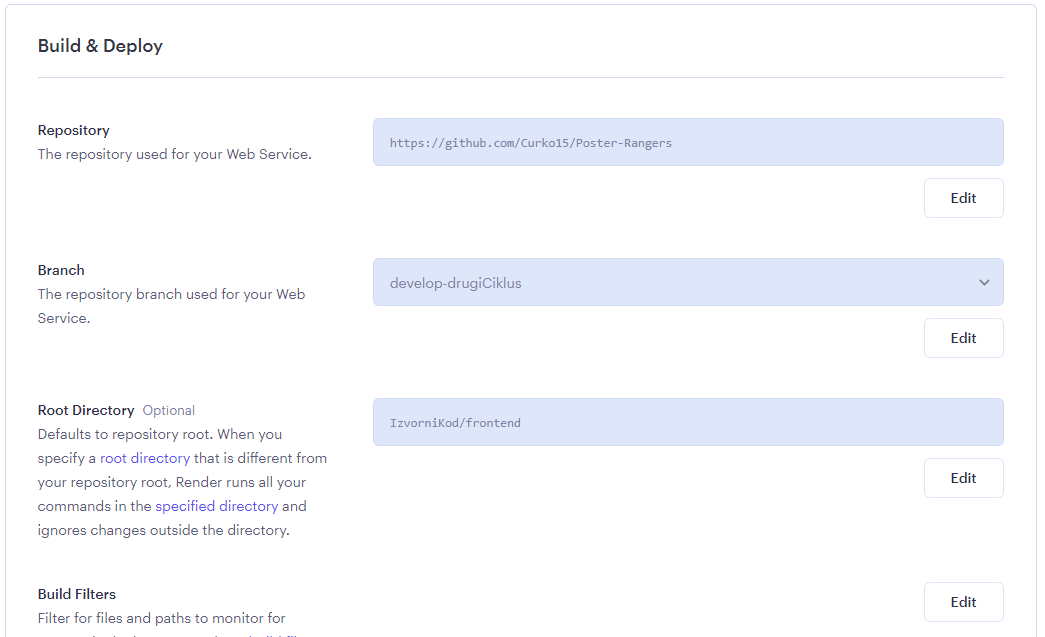
\includegraphics[width=\textwidth]{slike/FE_setup.png} %veličina u odnosu na širinu linije
				\caption{Postavljanje repozitorija, grane te direktorija za "frontend"}
				\label{fig:FE_setup} %label mora biti drugaciji za svaku sliku
			\end{figure}
			
			\begin{figure}[H]
				
\includegraphics[width=\textwidth]{slike/deployed_URL.png} %veličina u odnosu na širinu linije
				\caption{generirani URL za pristup puštenoj aplikaciji}
				\label{fig:deployed_URL} %label mora biti drugaciji za svaku sliku
			\end{figure}
			
			
			\eject 